% !TEX TS-program = pdflatex
% !TEX encoding = UTF-8 Unicode

%%% DOCUMENT DEFINITION
\documentclass[11pt, french]{article} % use larger type; default would be 10pt
\usepackage[utf8]{inputenc} % set input encoding (not needed with XeLaTeX)

%%% PAGE DIMENSIONS
\usepackage{geometry} % to change the page dimensions
\geometry{a4paper} % or letterpaper (US) or a5paper or....
\geometry{margin=2cm} % for example, change the margins to 2 inches all round

%%% PACKAGES
\usepackage{graphicx} % support the \includegraphics command and options
\usepackage{booktabs} % for much better looking tables
\usepackage{array} % for better arrays (eg matrices) in maths
\usepackage{paralist} % very flexible & customisable lists (eg. enumerate/itemize, etc.)
\usepackage{verbatim} % adds environment for commenting out blocks of text & for better verbatim
\usepackage{subfig} % make it possible to include more than one captioned figure/table in a single float
\usepackage{amsmath}
\usepackage[frenchb]{babel}

\usepackage{picins,caption}
\usepackage{wrapfig}
\usepackage{url}

%%% HEADERS & FOOTERS
%\usepackage{fancyhdr} % This should be set AFTER setting up the page geometry
%\pagestyle{fancy} % options: empty , plain , fancy

% Rapport projet pluridisciplinaire : etude thermique du pont en H
% : Xavier Galzin, Stanislas Bertrand, Romain Desille, Frédéric Meslin

\title{\textsc{Projet Pluridisciplinaire} \\ Solution Analogique \\
\begin{minipage}[c][20cm][c]{15cm}
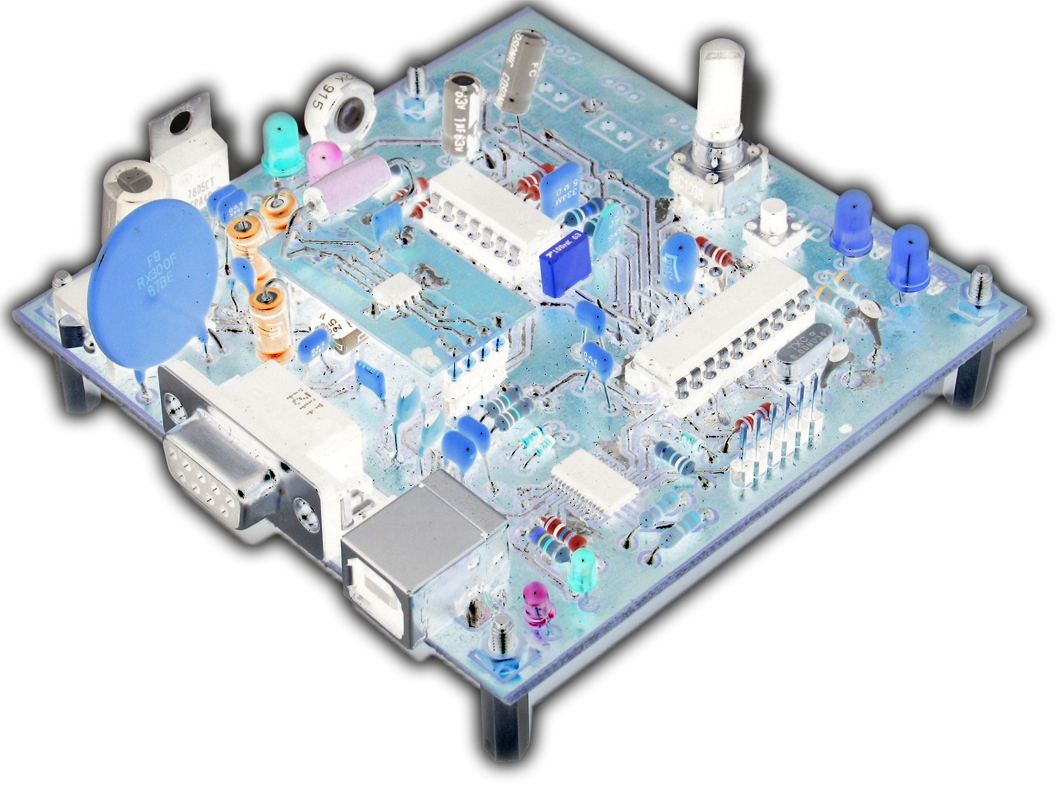
\includegraphics[width=15cm]{../Photos/CarteFrontInv.png}
\end{minipage}}
\author{Xavier GALZIN, Stanislas BERTRAND, Romain DESILLE, Frédéric MESLIN}
\date{\today}

\begin{document}
\maketitle

\pagebreak
\tableofcontents

\pagebreak
\section*{Introduction}

Dans le premier rapport, nous avons analysé le problème d'automatique soulevé par l'asservissement en position du mobile dans un équilibre instable. Grâce à des simplifications théoriques, nous avons pu mettre en place un modèle physique nous permettant de proposer un correcteur analogique adapté. 
Dans le rapport suivant, nous nous sommes intéressés à deux aspects relatifs à la partie numérique : la communication sérielle pour faciliter les réglages et permettre d'effectuer des mesures en temps réel et les mécanismes de conversion analogique / numérique puis numérique / analogique autant nécessaires pour la numérisation de la consigne et le pilotage de la puissance dans le cadre du correcteur analogique que pour la future solution à saveur plus numérique. 
\medskip

Ce présent rapport détaille la réalisation électronique de notre projet. Partant de la conception aux résultats des tests maquette effectués grâce au circuit imprimé gravé pour l'occasion, tous les modules impliqués dans le fonctionnement du prototype sont étudiés. Sont présentés dans l'ordre de la chaine de traitement de signal : la mise en forme des informations capteurs, l'implantation du correcteur analogique, la conversion de la consigne obtenue dans le domaine du numérique et enfin le pilotage du module de puissance pour répondre à cette problématique de lévitation.

%%%%%%%%%%%%%%%%%%%%%%%%%%%%%%%%%%%%%%%%%%%%%%%%%%%%%%%%%%%%%%%%%%%%%%%%%%%%%%%
% Capteur & Conditionnement -> Stan
%%%%%%%%%%%%%%%%%%%%%%%%%%%%%%%%%%%%%%%%%%%%%%%%%%%%%%%%%%%%%%%%%%%%%%%%%%%%%%%

\section{Capteur \& Conditionnement}
\subsection{Capteur à Effet Hall}


\subparagraph*{Principe du capteur à Effet Hall}~\\
\begin{minipage}[t]{10cm}
\vspace{-0.3cm}
\parpic{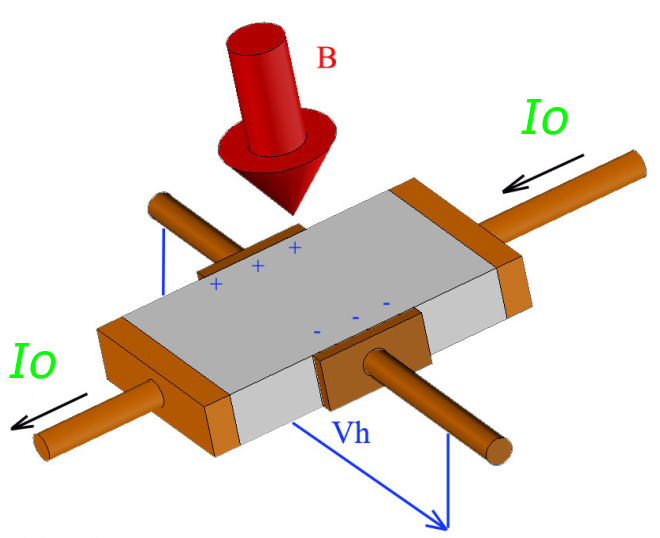
\includegraphics[width=5cm]{SolutionAnalogique/capteur_effet_hall}}
Un capteur à effet Hall permet de mesurer le champ magnétique $B$ grâce à la déformation d'un courant $I_0$ dans un conducteur ou semi-conducteur, soumis à ce champ. La déformation du flux d'électron génère une différence de potentiels aux bords du conducteur : $V_h =K_h \cdot B \cdot I_0$. Cette relation considère $B$ comme le champ magnétique normal à la surface du conducteur.
\end{minipage}


\subparagraph*{Implantation}~\\
\begin{minipage}[t]{10cm}
Pour mesurer les champs magnétiques de la bobine et du mobile deux capteurs à effet Hall (modèles Allegro A1302) sont placés à chaque extrémité de la bobine. L'alignement de la bobine, du mobile et des capteurs est important car c'est le champ magnétique normal au capteur qui est mesuré. Il est ainsi possible de connaitre la position verticale du mobile, les deux capteurs étant placés symétriquement sur la bobine, ils mesurent le même champ résultant. Le champ résultant du mobile n'est pas le même pour les deux capteurs, en effet, le champ diminue avec la distance. Le bilan des champs magnétiques exercés sur les capteurs est le suivant :
\vspace{-0.3cm} \[B_{H2} = B_{Bob} + B_{Mob~Dist_{Mob-H2}}\]
\vspace{-0.8cm} \[B_{H1} = B_{Bob} + B_{Mob~Dist_{Mob-H1}}\]
L'image de la position du mobile est contenue dans  $B_{Mob~Dist_{Mob-H2}}$ et $B_{Mob~Dist_{Mob-H1}}$. L'image est obtenue par différence de $B_{H2}$ et $B_{H1}$, $V_{H2}-V_{H1}$
\end{minipage}
~
\begin{minipage}[t]{8cm}
\vspace{-7cm}
\piccaption{Implantation des capteurs}
\parpic{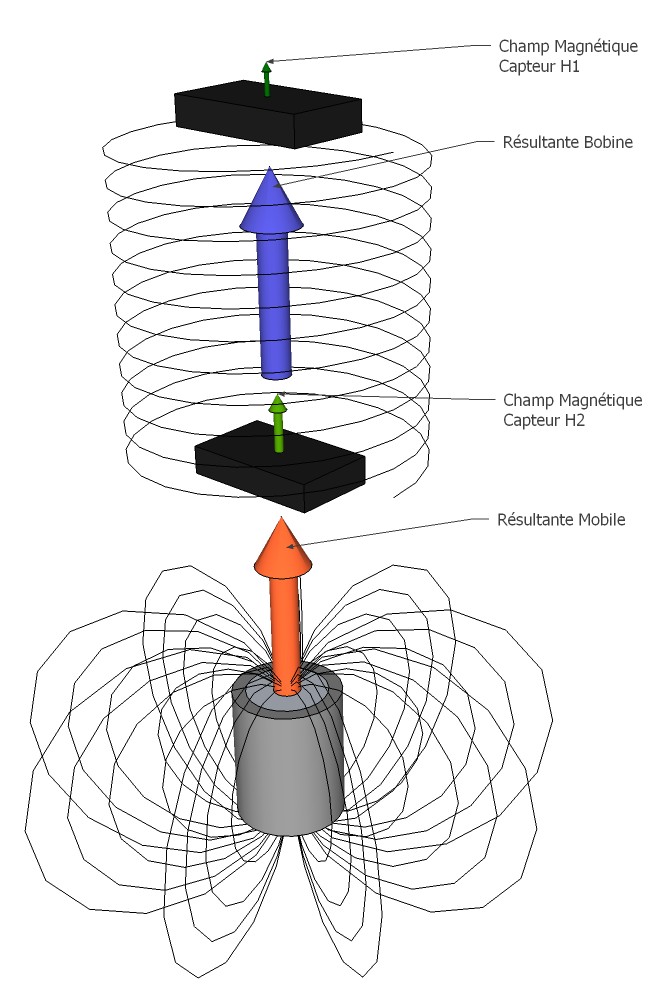
\includegraphics[width=8cm]{SolutionAnalogique/EffetHall}}
\end{minipage}


\subparagraph*{Caractéristiques électronique}~\\
Les capteurs Allegro A1302 conviennent à notre application car ils sont optimisés pour des systèmes de positionnement linéaires ou radiaux. Le capteur peut être alimenté par une tension de 5V, tension utilisé par nos montages analogiques. Le signal de sortie ne nécessite aucun conditionnement car la mesure effectuée est filtrée et amplifiée en interne et le niveau de sortie est directement compatible. Le circuit a une faible impédance de sortie, caractéristique importante pour les montages réalisés par la suite.

\subsection{Montage différentiel}

\begin{wrapfigure}{r}{8cm}
  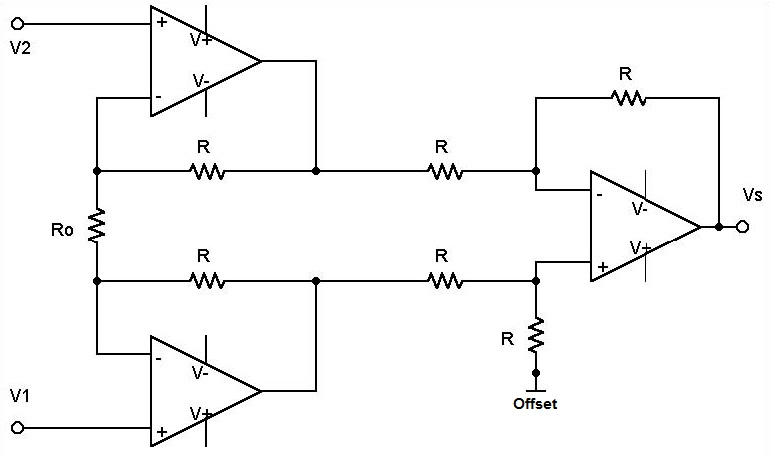
\includegraphics[width=8cm]{SolutionAnalogique/AmpInst}
  \caption{Amplificateur d'instrumentation}
\end{wrapfigure}
Le montage amplificateur d'instrumentation a été choisi pour son gain différentiel réglable, son taux de réjection en mode commun important grâce à l'étage d'entrée symétrique et ses impédances d'entrées fortes. De plus, ce montage a été spécifiquement développé pour notre type d'applications. D'autres montages soustracteurs plus simples, employant moins d'AOPs, auraient été envisageables mais l'économie de composants réalisée en regard des performances obtenues est discutable pour notre application. 

Un ensemble d'amplificateurs de type LM324 a été employé pour réaliser toutes les fonctions analogiques. Ce boitier a été choisi pour son aptitude à fonctionner en mono-tension, sa bande passante suffisamment élevée pour notre application et son caractère standard impliquant sa disponibilité. Un circuit LM324 comportant 4 AOPs identiques, il est tout indiqué pour l'implantation de l'amplificateur d'instrumentation.

Ce montage n'est pas réalisé de manière complètement intégrée ce qui dégrade ses performances, notamment à cause des imprécisions relatives des résistances $R$. Des composants idoines intégrant toute la structure existent et permettent des mesures de grande précision mais à un prix en rapport direct.

L'étude du schema donne la relation suivante : $V_s=(1+2 \frac{R}{R0})(V_1-V_2) + V_{offset}$. La mesure de la tension maximale de sortie permet de régler la valeur de l'offset, $V_{offset}=\frac{V_{max}}{2}$, $V_{max}=3.7$V. Cela permet de maximiser les variations du signal en le centrant dans la plage de sortie de l'AOP.

\subsection{Consigne Analogique}
\begin{wrapfigure}{r}{0.5\linewidth}
  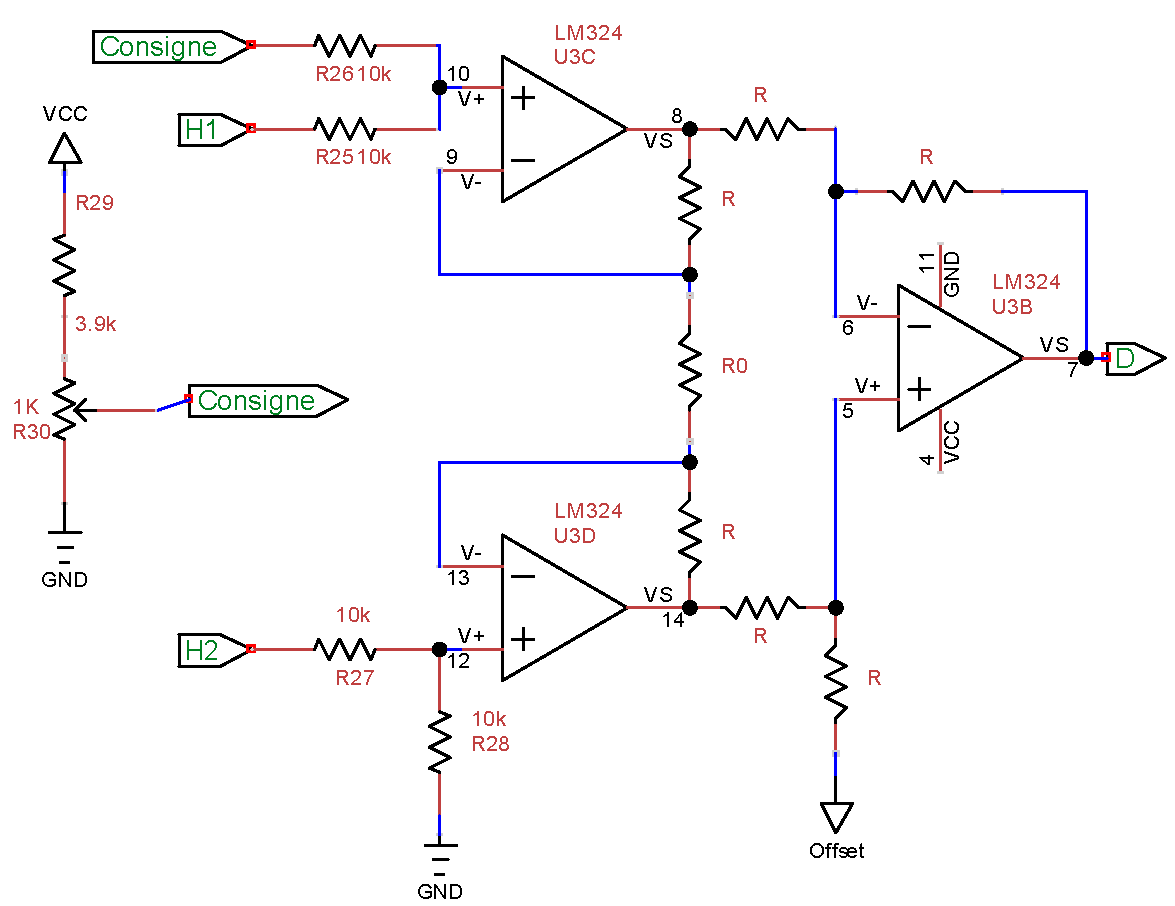
\includegraphics[width=\linewidth]{SolutionAnalogique/AmpInstCons.pdf}
  \label{DiffConsigne}  
  \caption{Différentiel avec consigne}
\end{wrapfigure}
La conception initiale ne prévoyait pas de consigne analogique, seulement une consigne numérique. Il s'est avéré plus intéressant d'ajouter une consigne analogique pour plusieurs raisons : elle permet de générer l'erreur et de travailler centré sur l'offset en sortie du montage différentiel. Cela permet de maximiser la plage du signal pour la numérisation.

La consigne est ajoutée en tirant avantage du montage différentiel. Désormais, sur l'entrée inverseuse du montage, deux signaux sont sommés, la consigne et le capteur $H1$. Le champ magnétique mesuré par $H1$ est plus faible que celui de $H2$ donc $H2-H1>0$. L'ajout de la consigne permet d'annuler cette tension pour une certaine position du mobile (position d'équilibre), la tension de sortie est alors celle de l'offset.
\begin{center}
$V_s=\frac{1}{2}(1+2 \frac{R}{R0})(H2-H1-Consigne) + V_{offset}$
$Consigne = (H2-H1)_{15mm}$
\end{center}
Le sommateur en entrée induit une division par deux des tensions. C'est pourquoi la tension du capteur H2 est également divisée via un pont. Cela est rendu possible grâce à la faible impédance de sortie des capteurs à effet Hall. La génération de consigne respecte cette contrainte, $R_{eq_{Consigne}} \ll R_{26}$. Pour faciliter le réglage, la course du potentiomètre a été fixée de 0 à 1V, ce qui est suffisant pour annuler $H2-H1$. Ce gain d'entrée est compensé par le gain du montage différentiel. 


%%%%%%%%%%%%%%%%%%%%%%%%%%%%%%%%%%%%%%%%%%%%%%%%%%%%%%%%%%%%%%%%%%%%%%%%%%%%%%%
% Correcteur Avance de phase
%%%%%%%%%%%%%%%%%%%%%%%%%%%%%%%%%%%%%%%%%%%%%%%%%%%%%%%%%%%%%%%%%%%%%%%%%%%%%%%


\section{Correcteur Avance de phase}

\subsection{Données}

\noindent
Pour le schéma et les formules (que nous avons quand même vérifiées) du correcteur, nous avions le choix entre deux montages différents que nous avons trouvé sur internet :



\begin{figure}[!h]
    \centering
    \begin{tabular}{cc}
      %\label{avph1}
     % \caption{Solution de correcteur 1}
      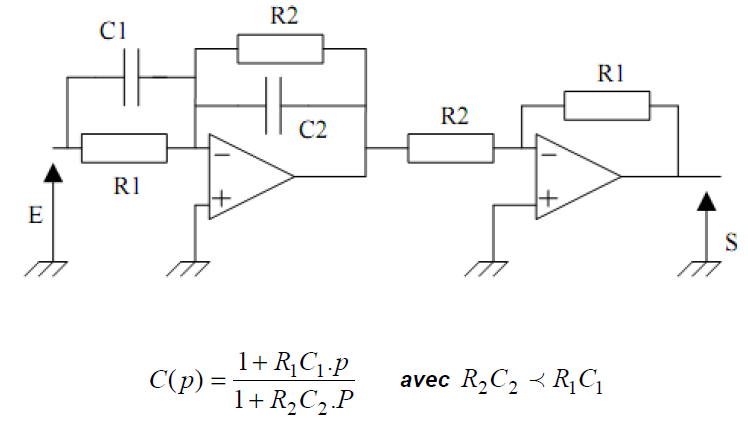
\includegraphics[width=8cm]{SolutionAnalogique/Avph.png} &
     % \label{avph2}
     % \caption{Solution de correcteur 2}
      \includegraphics[width=8cm]{SolutionAnalogique/Avph2.png} \\

      (a) & (b)\\
    \end{tabular}
    \caption{Légende: Deux solutions de réalisations analogiques pour le correcteur à avance de phase
    \label{avph_sol_poss}}
\end{figure}








Nous avons retenu le premier des deux schémas en raison de sa possibilité de régler plus facilement le rapport entre le zéro et le pôle. 


\subsection{Détermination de valeurs des composants}

Dans le schéma retenu, le produit $R_1*C_1$ correspond à la constante $ T_av$ définie dans le rapport d'automatique et le produit $R_2*C_2$ correspond à $0.1*T_av$. Nous allons déterminer les valeurs de $R_1$, $R_2$, $C_1$ et $C_2$ dans deux configurations : poids du mobile à $0.0897 kg$ correspondant à un $T_av$ de 0.0313 et poids du mobile à $0.1414 kg$ correspondant à un $T_av$ de 0.0393.

\vspace{0.5cm}

Pour des raisons de simplifications, nous prendrons les résistances $R_1$ et $R_2$ égales, le facteur 10 entre les constantes du numérateur et du dénominateur sera donc réalisé par un facteur 10 entre les valeurs des condensateurs. En outre, pour ne pas avoir à utiliser des condensateurs trop volumineux (pour des raisons de praticité vis-à-vis de la carte) et non polarisés, nous ne les prendrons pas de trop grandes valeurs et nous compenserons cela avec les résistances. Pour le poids de $0.0897 kg$, en choisissant des composants avec des valeurs normalisées, on obtient ainsi $R=100.0 K\Omega$, $C_1=330 nF$ et $C_2=33 nF$.

\vspace{0.5cm}
On fera plutôt varier les résistances que les condensateurs pour s'adapter au changement de poids. On conserve donc les mêmes valeurs de condensateurs. On trouve alors $R=119.090 K\Omega$ pour pouvoir gérer le changement de poids. Il sera donc possible de prendre des potentiomètres pour ajuster les constantes, corrigeant ainsi les écarts possibles des valeurs de condensateurs. Dans la pratique, on fera plutôt varier le gain du montage pour compenser le changement de poids. 

\vspace{0.5cm}

Nous avons cependant apporté une modification en enlevant le deuxième AOP pour des raisons d'économie. Cela cause juste l'apparition d'un facteur $\frac{-R2}{R1}$. Les résistances étant égales, la seule différence que cela fait est un signe "-" que nous compenserons grâce au microcontrôleur. Le schéma final du correcteur à avance de phase est donc le suivant :

\begin{figure}[!h]
    \centering
	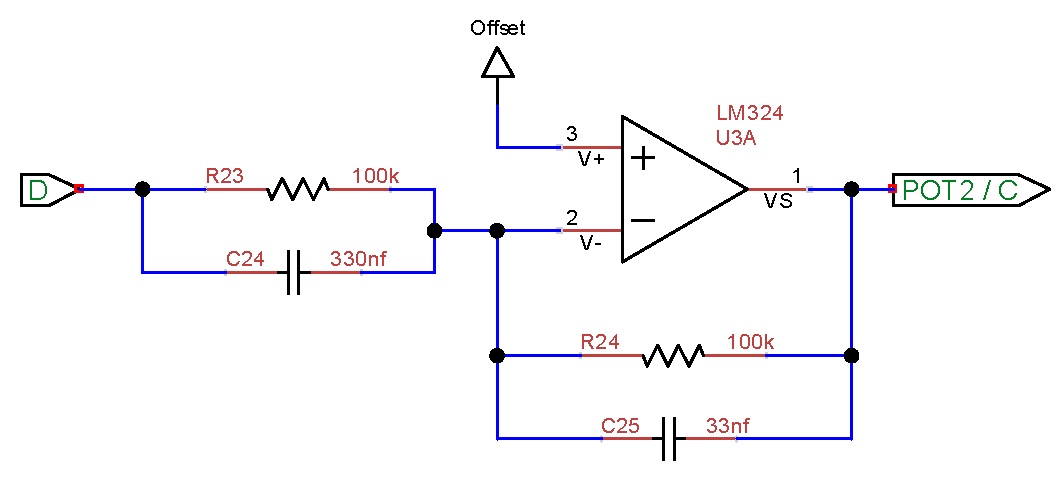
\includegraphics[scale = 0.8]{SolutionAnalogique/AvPhase.pdf}
	\label{avph_schm}
	\caption{Schémas retenu pour le correcteur à avance de phase}
\end{figure}

Aussi, par le biais de MATLAB, nous avons pu obtenir la courbe théorique de notre correcteur par avance de phase :

\begin{figure}[!h]
    \centering
	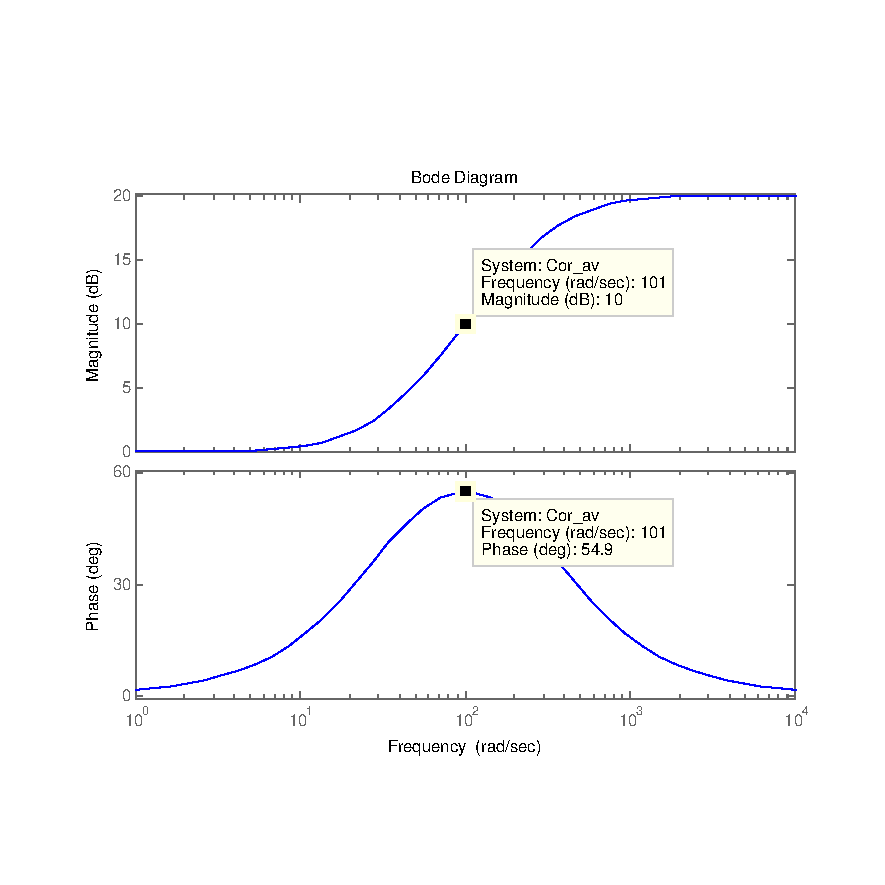
\includegraphics[scale = 0.8]{SolutionAnalogique/BodeAvPhase.pdf} 
	\label{avph_bode}
	\caption{Diagramme de gain et de phase du correcteur (Matlab)}
\end{figure}


A noter que la fréquence donnée est en $rad.s^-1$, elle vaut environ 16 Hz et correspond bien au pole du correcteur calculé lors de la partie automatique. On observe un gain de 10 dB à la fréquence où l'on travaillera et dont il faudra tenir compte pour la suite. 



\subsection{Validation par simulation PSpice}

On simule le correcteur à avance de phase par le schémas suivant : 

\begin{figure}[!h]
    \centering
	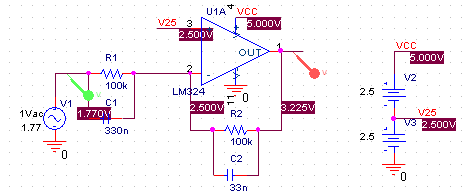
\includegraphics[scale = 0.8]{SolutionAnalogique/orcad_sch.png} 
	\label{avph_schm_simu}
	\caption{Schémas de test utilisé pour la simulation avec Orcad}
\end{figure}

On obtient le résultat de simulation suivant : 

\begin{figure}[!h]
    \centering
	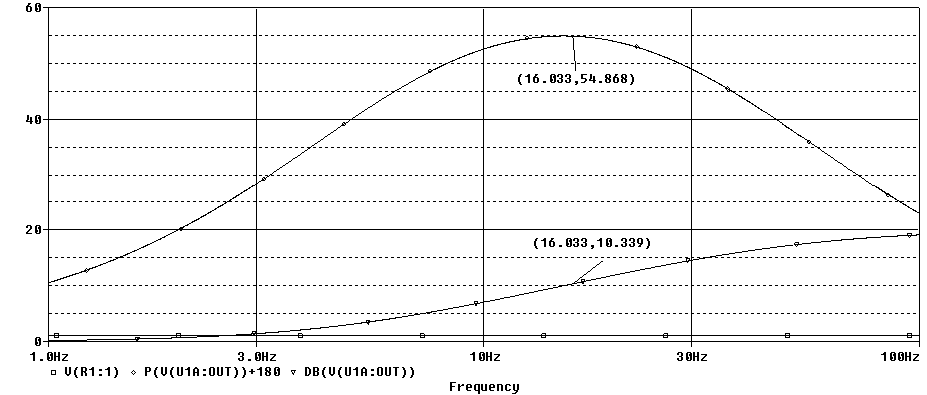
\includegraphics[width = 15cm]{SolutionAnalogique/orcad_simu.png} 
	\label{avph_schm_simu_res}
	\caption{Diagramme de gain et de phase du correcteur (Orcad)}
\end{figure}


Comme on peut le voir en comparant par rapport au résultat donné par MATLAB, le schéma répond comme on le souhaitait. 

\vspace{0.5cm}
\subsection{Conclusion de l'étude théorique}

\noindent
Nous avons donc validé notre choix de montage de correcteur et nous avons déterminé des valeurs admissibles de composants analogiques grâce à cette étude. Il faudra cependant être attentif quant au choix des condensateurs vis-à-vis de leur fréquence de fonctionnement.  

\subsection{Validation du modèle câblé}

\vspace{0.5cm}

\begin{figure}[!h]
    \centering
	\includegraphics[width = 10cm]{SolutionAnalogique/avph_reel.png} 
	\label{avph_reel}
	\caption{Résultat observé du correcteur à avance de phase}
\end{figure}

Comme on peut le voir sur cette photo où l'on à réglé un signal d'entrée de 16Hz , on a bien un gain de 10dB (gain d'environ 3) : tension d'entrée (CH2) à 1V, tension de sortie (CH1) à environ 3V. Au niveau du déphasage, on a un carreau d'écart pour une période de 6.2 carreau ce qui correspond bien à un déphasage de 60\char23 attendu. 


\section{Conversion \& Communication}
\subsection{Choix du microcontrôleur}

Tout d'abord, nous voulions utiliser un microcontrôleur de la famille des PIC puisque nous étions davantage habitués à leur programmation et que nous avons toujours eu une bonne expérience avec ces composants.  %de l'aversion totale de tous les membre du groupe à l'égard des microcontrôleur TI (surement causée par le cours génialissime de M.Nezan en 3ème année). 
%
%\vspace{0.5cm}
%
%Une fois ce choix fait, nous avons recherché le microcontrôleur qui nous éviterait le maximum de contraintes par la suite. C'est pour cela que nous avons choisi le PIC24FV32KA301. Celui-ci dispose d'un régulateur interne qui génère une tension 3.3V à partir du 5V de l'alimentation externe. Il nous épargne donc la partie adaptation de tension. 
%
%\vspace{0.5cm}
%
%En outre, nous voulions un microcontrôleur assez rapide pour supporter les calculs complexes que nous aurons surement à faire lors de la partie sur la correction numérique. Ainsi, la fréquence de travail de notre microcontrôleur est de 16 MHz en interne et il dispose de module de multiplication et de semi-division (1 cycle pour une multiplication et 19 pour une division). 
%
%\vspace{0.5cm}
%
%Enfin, notre microcontrôleur dispose d'un CAN 12 bits qui sera utile lors de la programmation et d'un module UART qui nous servira lors de la mise en place de la communication série. Disposant déjà des outils de développement Microchip, nous ne perdrons pas de temps à l'installation de ces derniers. 


%Nous voulions travailler avec les produits de Microchip, ce choix c'est fait par habitude car nous avions déjà tous utiliser les produits Microchip et nous n'avions eu aucun problème avec ces composants. Avant tout, nous avons fait la liste des caractéristiques du microcontrôleur dont nous avions besoin.

\begin{itemize}
	\item \textbf{Tension d'alimentation}
	Nous avons fait le choix d'uniformiser les tensions d'alimentation du microcontrôleur, des capteurs et du convertisseur "Serie/USB" afin de se passer d'adaptation en tension. C'est pourquoi l'intégralité de la carte est alimenté en 5V, le microcontrôleur contenant un régulateur interne qui génère le 3.3V dont il a besoin en interne.
\vspace{0.5cm}
	\item \textbf{Fréquence de travail}
	Afin de nous donner une certaine liberté concernant les calculs entre chaque échantillonnage des valeurs de capteurs, nous avons opté pour un microcontrôleur pouvant fonctionner à 32MHz. Les microcontrôleurs Microchip utilisant deux cycles d'horloge par instruction, nous avons donc un microcontrôleur fonctionnant à 16 MIPS. 
\vspace{0.5cm}
	\item \textbf{Conversion Analogique/Numérique}
 	Nous avons fait le choix de multiplier les points d'acquisitions, nous voulions pouvoir obtenir l'image numérique des capteurs, de la tension de sortie du montage différentielle et de celle du correcteur. Nous voulions donc un microcontrôleur possédant au minimum 4 entrées permettant la conversion analogique/numérique.
\vspace{0.5cm}
	\item \textbf{PWM et Timers} 
	Nous n'avions pas énormément de contraintes concernant la génération du PWM. Les microcontrôleurs 16 bits Microchip possédant des timers dédiés pour chaque sortie de comparaison (PWM), nous avions seulement besoin d'une sortie "OutputCompare".
\vspace{0.5cm}
	\item \textbf{Multiplicateur/Diviseur hardware}
	Afin de minimiser le temps de calcul de la solution numérique, nous avons cherché un microcontrôleur possédant un multiplieur/diviseur hardware. Cela qui diminuera la temps de calcul entre chaque échantillonnage de façon non négligeable (1 cycle pour une multiplication et 19 pour une division).
\vspace{0.5cm}
	\item \textbf{Outils de développement}
	Comme nous possédions déjà un programmateur Microchip : Pickit 3. Nous avons chercher un microcontrôleur supportant la programmation et le débogage par Pickit 3.
\vspace{0.5cm}
\end{itemize}

Nous avons donc cherché un microcontrôleur répondant à ces impératifs. Nous avons trouvé le PIC24FV32KA301 ayant les caractéristiques suivantes :
\begin{itemize}
\item \textbf{Tension d'alimentation :} entre 2V et 5,5V
\vspace{0.5cm}
\item \textbf{Fréquence de travail :}jusqu'à 32Mhz
\vspace{0.5cm}
\item \textbf{Conversion Analogique/Numérique :}convertisseur analogique/numérique 12 bit différentiel , 12 entrées, 100kSa/s échantillons par seconde. 
\vspace{0.5cm}
\item \textbf{PWM et Timers :}3 Output Compare, résolution 16 bits
\vspace{0.5cm}
\item \textbf{Multiplicateur/Diviseur hardware :}multiplieur hardware 16x16 bits, semi-diviseur hardware 32x16 bit
\vspace{0.5cm}
\item \textbf{Outils de développement :} Pickit3 supporté

\end{itemize}

\subsubsection{Conversion A/D}

Le module ADC offert par notre microcontrôleur comprend deux voies d'acquisition multiplexables avec un cycle d'échantillonnage-conversion relançable automatiquement. Dans notre cas nous utiliserons la voie A et le Timer1 génèrera l'événement qui déclenche le passage d'échantillonnage à conversion périodiquement et automatiquement (fréquence de l'évènement du Timer1 réglée à 1 kHz). L'échantillonnage reprendra dès la conversion terminée et le format des résultats sera en décimal sans signe puisque nous mesurons une tension qui sera entre 0 et 5V. 

\vspace{0.5cm}

Ne reste plus qu'à régler la fréquence à laquelle ces cycles d'échantillonnage-conversion vont se répéter. Dans notre cas, nous avions déterminé dans le rapport sur la partie automatique qu'une fréquence d'1 kHz serait suffisante. 

\vspace{0.5cm}

Après quelques tests, il apparait que l'échantillonnage le plus lent que l'on puisse faire est de période 992$\mu$s. En effet, on a $T_{AD} = (ACDS+1) * T_{CY}$ avec $T_{CY} = \frac{2}{F_{OSC}}$, $F_{OSC}$ étant la fréquence du microcontrôleur avant passage dans le module des PLL donc 8 MHz. On a donc $T_{CY} = 500 ns$ et en prenant le maximum d'ADCS qui vaut 63, on a $T_{AD} = 64 * T_{CY} = 32 \mu s$. Ensuite, on peut déclencher chaque cycle d'échantillonnage tout les $SAMC * T_{AD}$. En prenant le maximum de SAMC (soit 31), on obtient finalement $T_{samp} = 31 * T_{AD} = 992 \mu s$, ce qui est très proche de ce que l'on visait.  

\vspace{0.5cm}

Une fois la phase d'initialisation effectuée, la fonction qui récupère l'échantillon se compose simplement d'une sélection de la voie et d'une attente active sur le flag de fin de conversion. On récupère et on retourne la donnée convertie à l'issue de cette attente. 

\vspace{0.5cm}

L'attente active n'est pas gênante puisque l'on récupère la valeur de l'échantillon à chaque début d'interruption sur le Timer 1 et que la conversion, qui est très rapide à effectuer, à déjà débuté dès lors que l'on a généré le signal d'interruption du Timer 1. On enchaine ensuite avec la suite du programme pendant que l'échantillonnage reprend et on termine normalement largement avant la prochaine interruption.

\vspace{0.5cm}

%Les codes C correspondant à la fonction d'initialisation et à la fonction de récupération d'un échantillon pourront être trouvés en annexe. 

\subsection{PWM - Pulse Width Modulation}

Chaque sortie PWM du microcontrôleur possèdent un Timer dédié ce qui permet de ne pas monopoliser un Timer pour générer la sortie PWM.

Pour configurer le Timer OC1 (Output Compare 1), il faut tout d'abord choisir le mode de fonctionnement du Timer. Nous avons choisi d'utiliser le Mode "EDGE-ALIGNED PWM".

\begin{figure}[!h]
	\centering
	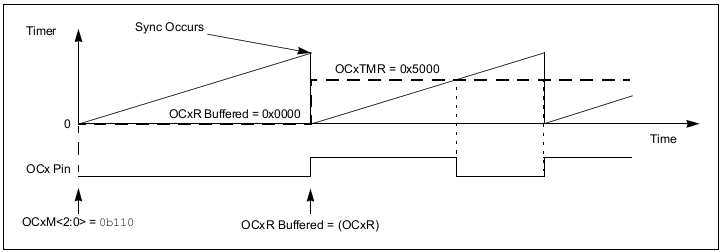
\includegraphics[width = 15cm]{SolutionAnalogique/PWMMode.png} 
	\label{pwm_mode}
	\caption{Schémas de principe du mode EDGE-ALIGNED PWM}
\end{figure}

Nous avons ensuite réfléchi à l'ordre de grandeur de fréquence de la PWM. Cette dernière ne doit pas être inférieure à 30 kHz, un fréquence inférieure risquerait de générer des fréquences audibles et donc d'engendrer un bruit avec de la bobine. Il ne faut pas non plus que la fréquence de la PWM soit trop élevée, sinon la résolution du rapport cyclique deviendrait trop faible.

Nous avons trouvé par le calcul le bon compromis : 62 kHz. Cela nous donne une résolution de 8 bits pour le rapport cyclique en utilisant Fcy comme horloge d'entrée Fcy étant la fréquence de cycle.
\begin{center}
$F_osc = 32MHz$
\\$F_cy = Fosc/2 = 16MHz$
\\$F_PWM = 16MHz/2^8 = 62,5kHz$
\end{center}
\vspace{0.5cm}

%Les codes C correspondant à la fonction d'initialisation et à la fonction de récupération d'un échantillon pourront être trouvés en annexe. 

\section{Contrôle de la puissance}

	La génération de la puissance dans notre application est une partie critique. Faire léviter un mobile d'un poids d'une centaine de gramme soumis à la gravité nécessite l'emploi d'une bobine de taille importante en comparaison avec les selfs classiquement rencontrées dans les montages électroniques. L'objectif est de produire un champ magnétique puissant pour porter le mobile. Ceci implique la régulation de courants importants, naviguant autour de deux ampères. 

\subsection{Choix d'un pont complet}
	Pour contrôler le champ magnétique émis, nous avons opté pour le pilotage de la bobine en tension. Étant donné la forte intensité des courants invoqués et pour éviter un trop grand gaspillage énergétique, le cahier des charges imposait une régulation en commutation plutôt qu'en fonctionnement linéaire. La bobine étant d'inductance élevée et de résistance faible, elle forme donc un filtre passe bas :

\medskip
$ L_{bob} = 14,9 mH $
$ R_{bob} = 2.24 \Omega $

\medskip
En considérant l'impédance de sortie du générateur de tension négligeable, on obtient :

$ F_{coupure} = \dfrac{1}{2\pi \times R_{bob} \times L_{bob}} = 4.77 Hz $

\medskip
Ce circuit constitue un filtre passe bas pour le courant d'une fréquence de coupure très faible. Nous allons donc pouvoir piloter la bobine à l'aide de PWMs ou MLIs (Modulation de largeur d'impulsion) à des fréquences relativement élevées. Le filtre réalisé lissera ensuite les impulsions pour former un courant continu proportionnel au rapport cyclique employé.

\medskip
\noindent
Pour générer les impulsions de tension, nous avions le choix entre trois solutions :

\medskip
\begin{itemize}
	\item \textbf{Transistor simple :} solution basique permettant d'alimenter ou non la bobine et de faire circuler le courant dans un seul sens.
	\item \textbf{Demi pont en H :} solution intermédiaire permettant de faire circuler le courant dans les deux sens mais nécessitant une source d'alimentation de puissance négative.
	\item \textbf{Pont en H complet :} solution ultime permettant de faire circuler le courant dans les deux sens sans disposer d'une source d'alimentation de puissance négative.
\end{itemize}

\begin{figure}[h!]
\centering
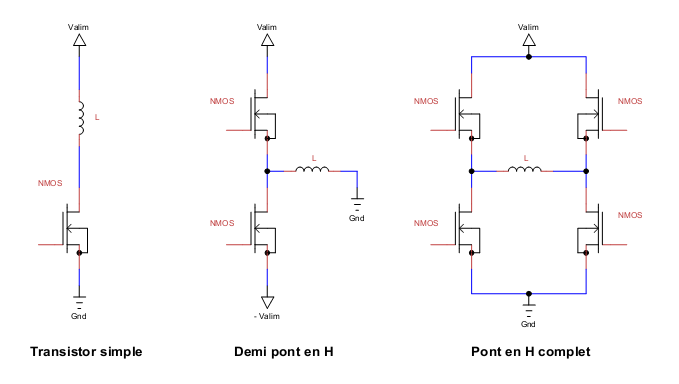
\includegraphics[width = 15cm]{SolutionAnalogique/Ponts.png} 
\caption{Différentes solutions de distribution de la puissance}
\end{figure}

Nous avons supposé que la possibilité d'inverser le sens du courant dans la bobine pouvait être intéressante pour notre application et ayant pour contrainte de conception la présence d'une seule source d'alimentation de puissance, nous avons sélectionné la solution du pont complet. Après discussion avec des encadrants du projet, nous avons émis l'hypothèse que la répulsion de la bobine pourrait améliorer la stabilité de l'asservissement et la consommation électrique globale du système. Ce qui semble certain c'est qu'elle facilite le positionnement manuel initial du mobile. Nous pourrons par la suite affirmer ou infirmer ces hypothèses en contraignant ou non le pont à fonctionner dans un seul sens. Nous saurons donc si le choix du pont complet était judicieux. Cette solution à l'inconvénient majeur d'être largement plus onéreuse à mettre en place que la première solution à un seul transistor.

\subsection{Choix du composant intégré}

Contrairement au circuit faisant la mesure différentielle des informations capteurs, nous avons préféré l'emploi d'une technologie intégrée pour réaliser le pont. Les avantages de cette solution sont multiples : les transistors de puissance sont optimisés pour cette application, leur circuit de pilotage est intégré et on dispose de protections à la fois thermiques et par mesure de courant circulant dans la bobine.

\medskip
\noindent
Nous avons choisi le circuit Allegro (A4950) possèdant les caractéristiques suivantes :
\medskip
\begin{itemize}
	\item Tension maximum de puissance $ V_{max} = 40 V $
	\item Courant maximum de puissance $ I_{max} = 3.5 A $, tolérance de pics à $ I_{peak} = 6.0 A$
	\item Faible $R_{DS_{on}} = 0.8 \Omega $ maximum @ $ T_j = 25 \char23 C $ \newline
	et $R_{DS_{on}} = 1.3 \Omega $ typique @ $ T_j = 125 \char23 C $
	\item Niveaux logiques d'entrée compatibles avec logique 0 - 5V
	\item Boitier miniature CMS SOICN 8 avec pad thermique
\end {itemize}

\begin{figure}[h!]
	\centering
	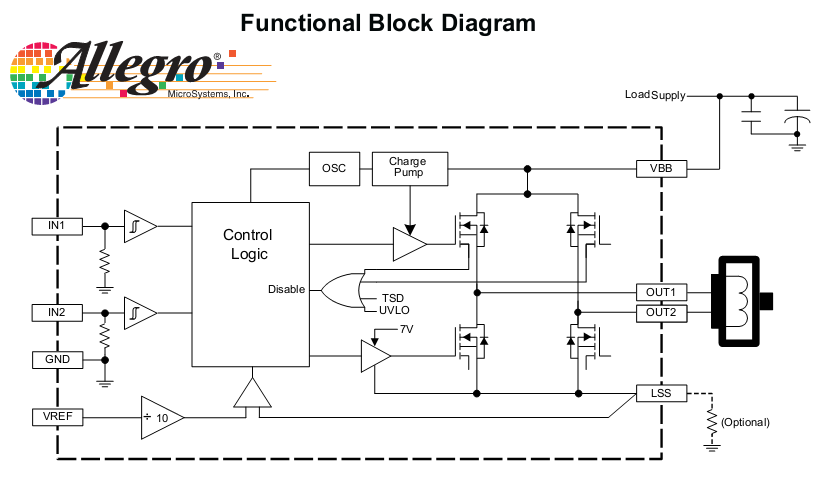
\includegraphics[width = 15cm]{SolutionAnalogique/A4950.png} 
	\caption{Schéma bloc interne du composant}
\end{figure}

\medskip
Le schéma interne précise les différents modules intégrés au composant. Le bloc \emph{control logic} pilote les grilles des transistors MOS de puissance par l'intermédiaire d'amplificateurs. On remarque la présence d'une pompe de charge pour générer une tension positive supérieure à la tension présente sur $ V_{VBB} $ car tous les transistors du pont sont des MOSFET à canal N. Un dispositif de comparateur permet d'implanter une limitation de courant dans le pont. Il fonctionne en comparant la tension présente sur $ V_{LSS} $ avec la tension de référence $ V_{REF} $ après une division par 10. Nous avons donc ajouté une résistance de mesure et de puissance de $ 0.1 \Omega $. Ceci nous donne une correspondance directe entre la tension de référence et le courant maximum autorisé dans le pont.

\begin{figure}[h!]
	\centering
	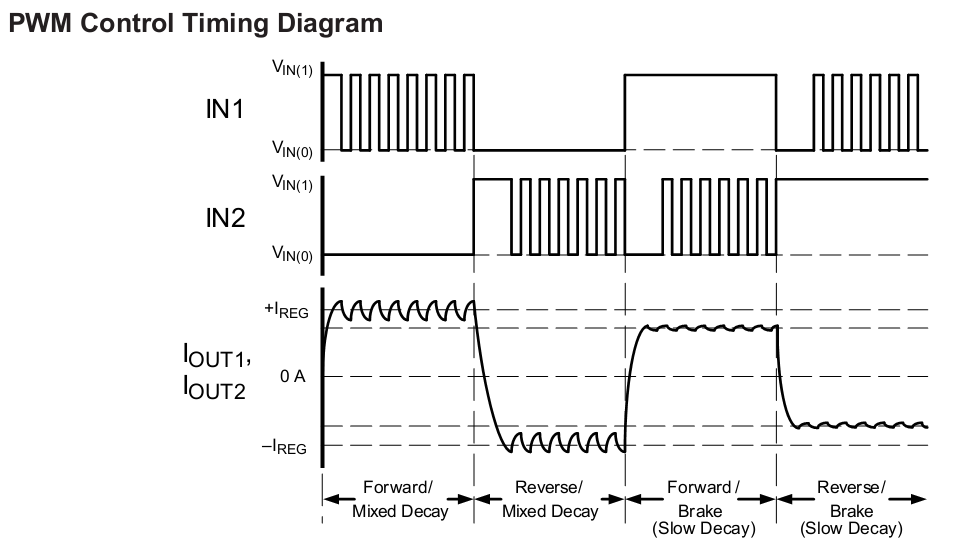
\includegraphics[width = 15cm]{SolutionAnalogique/PWMtimings.png} 
	\caption{Modes de fonctionnement du circuit}
\end{figure}

Ce diagramme illustre les différents modes de fonctionnement du circuit. On en retiens deux modes utiles pour notre application : le mode forward et reverse. Les deux autres modes sont des modes de freinage, utilisés pour la commande de moteurs à courant continu. Pour alimenter notre bobine dans un certain sens, il suffit de piloter l'une des entrées $ IN_1 $ ou $ IN_2 $ et de forcer l'autre à la masse. Nous n'avons donc eu besoin que d'une sortie PWM sur notre microcontroleur pour contrôler entièrement le pont.

\medskip
En plus de ses bonnes caractéristiques électriques et de son pilotage aisé, ce circuit est disponible au catalogue Farnell et fait partie des composants les moins chers. En le choisissant, nous avons quand même négligé deux aspects qui ont débouché sur des difficultés d'intégration importantes : la taille réduite du boitier (SOICN 8) et la nécessité d'un bon dispositif de dissipation thermique pour le refroidir.

\subsection{Analyse de la dissipation thermique}
Avant de réaliser la carte fille intégrant le pont nous avons fait une étude de dissipation thermique. Cet aspect était nécessaire pour concevoir le circuit imprimé en conséquence.

\subsubsection{Caractéristiques thermiques}
Les données techniques composants sont les suivantes :

\medskip
\noindent
$ R_{TH} = 62 \char23C.W\up{-1} $ : résistance thermique du boitier \newline
$ T_{JUNC\_{MAX}} = 160 \char23C $ : température maximale de la jonction \newline
$ T_{AMB} = 25\char23C $ : température ambiente considérée \newline
$ R_{DSON\_{MAX}} = 1.3 \Omega $ : résistance drain - source interne \newline
\noindent

On ne peut que constater que la valeur de $ R_{DSON\_{MAX}} $ est élevée en comparaison à celle de bon transistors MOS discrets. Cette caractéristique est discriminante pour le rendement et permet le calcul la puissance perdue par effet Joule. La valeur de $R_{TH}$ est donnée par le fabricant pour une dissipation de la chaleur dans un circuit imprimé deux couches, de 0.8 mm d'épaisseur et suffisament étendues. Dans le cas d'une conception à 4 couches, cette valeur peut descendre jusqu'à $ 35 \char23C.W\up{-1} $.

\subsubsection{Analyse de l'échauffement}

\noindent
L'équation de la température de la jonction est donnée par : \newline
\medskip
\noindent
$ T_{JUNC} = R_{TH} * P_{DIS} + T_{AMB} $

\medskip
\noindent
Si on considère que le courant moyen distribué par le pont vaut : \newline
$ I_{MOY} = 1.28 A $

\medskip
\noindent
On obtient la puissance dissipée par le composant : \newline
$ P_{DIS} = R_{DSON} * I_{MOY}\up{2} = 1.3 * 1.28\up{2} = 5.2 W $

\medskip
\noindent
Et par conséquence la température de la jonction en fonctionnement : \newline
$ T_{JUNC} = R_{TH} * P_{DIS} +  T_{AMB} = 62 * 5.2 + 25 = 157 \char23 C $

\subsubsection{Conclusion de l'étude thermique}

	On constate que le résultat trouvé est très proche de la valeur limite de la température de jonction $ T_{JUNC\_{MAX}} $ du composant. Cependant, nous avons effectué le calcul dans le pire des cas et on pouvait présumer que cette situation ne sera pas atteinte.

\subsection{Réalisation de la platine de puissance}
Pour intégrer notre pont complet dans la chaine de commande, nous avons réalisé une platine fille dédiée s'enfichant sur le circuit imprimé. L'intérêt était de pouvoir changer de composant de puissance au cas où la dissipation n'était pas suffisante pour le faire fonctionner. Le fait que la platine soit surélevée par rapport à la carte mère améliorait aussi son aération et donc sa dissipation.

La plupart des composants de gestion de puissance sont intégrés dans des boitiers imposants, possédant des surfaces métaliques permettant une dissipation de la chaleur améliorée (TO 220, pentawatt, S0T23 ...). On trouve aussi des composants en boitier DIP avec des pattes, en général deux paires situées au centre, prévues pour évacuer la chaleur . La technologie de dissipation de notre pont est tout autre : le boitier utilisé est de type SOIC standard à la différence qu'il comporte un \emph{pad thermique} relié au substrat du circuit et situé en dessous du composant. L'objectif est de dissiper la chaleur produite dans les différentes couches de cuivre avoisinantes. Les illustrations de la datasheet du A4950 conseillent l'utilisation de vias pour répartir la chaleur dans les circuits imprimés multicouches et proposent un layout particulier.

\begin{figure}[h!]
	\centering
	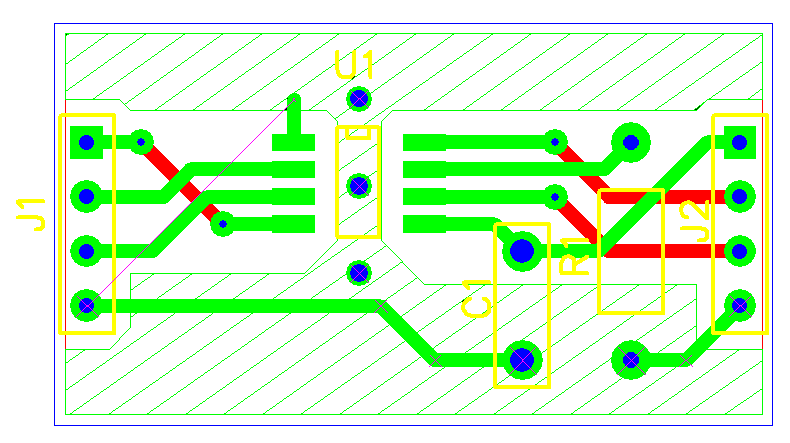
\includegraphics[width = 15cm]{SolutionAnalogique/Layout.png}
	\caption{Le circuit imprimé de la carte fille}
\end{figure}
Le circuit imprimé réalisé possède deux plans de masse destinés à dissiper un maximum de chaleur. Le plan inférieur couvre quasiment toute la surface de la plaque et le plan supérieur est représenté par la surface hachurée verte. Trois vias servent à assurer la conduction thermique entre les plans.

\subsection{Utilisation du four à refusion}
Pour souder le circuit AL4950 et notamment le pad thermique, nous avons utilisé un four à refusion. La datasheet ne proposant pas de consigne de température, nous avons utilisé une consigne par défaut. Le four nous a permis d'assurer une conduction thermique suffisante entre le pad et la surface cuivrée.

\begin{figure}[h!]
	\centering
	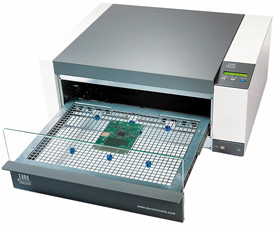
\includegraphics[width = 8cm]{SolutionAnalogique/fourarefusion.jpg}
	\caption{Le four utilisé pour souder le pont}
\end{figure}

\subsection{Changement du composant de puissance}
Avec notre pont complet nous avons réussi à faire léviter le mobile. D'abord la partie aimanté seule, ensuite avec le leste. Nous avons constaté que l'échauffement était important, que la dissipation faite par le circuit imprimé était relativement bonne mais en définitive insuffisante. Après règlages, nous avons réussi à respecter le cahier des charges avec la partie aimantée seule mais pas avec le mobile leste. Au delà d'une distance de lévitation de 14 mm, l'échauffement était trop élevé et la protection thermique du circuit se déclenchait innopinément faisant chuter le mobile. La consommation de courant était mauvaise à cause de la forte valeur de $ R_{DSON} $.

\begin{figure}[h!]
	\centering
	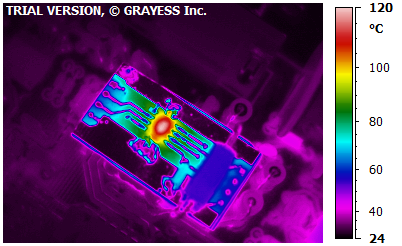
\includegraphics[width = 8cm]{SolutionAnalogique/VueThermique.png}
	\caption{Vue du pont en fonctionnement avec caméra thermique}
\end{figure}

Nous avons donc essayé d'améliorer la dissipation en

\section{Résultats - Evolution}

\subsection{Prix de la solution}
Nous avons fait une rapide évaluation du prix de notre solution. Pour se faire, nous avons pris en compte les prix pour 1 et pour 500 pièces de Farnell. On obtient ainsi une fourchette relativement large qui permet de se donner une idée du coût de notre solutions selon le contexte (production intensive ou prototype). Le prix trouvé est d'environ 19 euros pour les composants seuls avec les prix pour 1000 et d'environ 32 euros pour les composants seuls avec les prix pour 1. Étant donné la taille de notre carte, nous évaluons à 8 euros les coûts concernant l'achat de la carte et le routage dans le cas d'une production massive et à 12 euros dans le cas de la conception d'un prototype. Cela amène le prix total à une fourchette de 27 à 44 euros selon le type de production. Il est certain que ce prix peut descendre en n'utilisant pas un pont complet et en trouvant une alternative moins onéreuse au FT232. 

 
Le détail du prix des composants pourra être trouvé en annexe. 

\section{Conclusion}

%
%\pagebreak
%\section{Bibliographie}
%\medskip
%- Cours de GEE, A. Meghebbar :
%\newline \textit{\underline{\url{fsi.univ-tlemcen.dz/cours/Support-Cours-Commande-Analogique-Master-Electrotechnique10.pdf}}} 
%
%- Cours de systèmes asservis linéaires, Jean Philippe MULLER : 
%\newline \textit{\underline{\url{http://www.ta-formation.com/cours-sal/n-sal.pdf}}} diapo 28
%
%- Cours sur les amplificateurs d'instrumentation, Olivier FRANÇAIS : 
%\newline \textit{\underline{\url{http://www.esiee.fr/~francaio/enseignement/version_pdf/III_amplidiff.pdf}}} page 13
%
%
%\pagebreak
%\section{Annexe}
%\medskip
%\begin{figure}[!h]
%	\centering
%	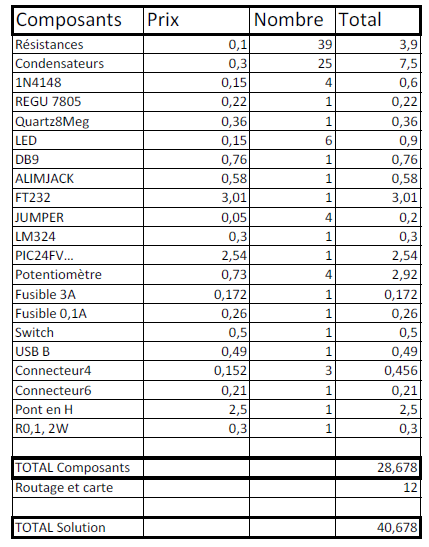
\includegraphics[width=10cm]{SolutionAnalogique/cout.png}
%	\label{cout}
%	\caption{Tableau répertoriant les composants utilisés et leurs coûts}
%\end{figure}

\pagebreak
\section{Bibliographie}
\medskip
- Cours de GEE, A. Meghebbar :
\newline \textit{\underline{\url{fsi.univ-tlemcen.dz/cours/Support-Cours-Commande-Analogique-Master-Electrotechnique10.pdf}}} 

- Cours de systèmes asservis linéaires, Jean Philippe MULLER : 
\newline \textit{\underline{\url{http://www.ta-formation.com/cours-sal/n-sal.pdf}}} diapo 28

- Cours sur les amplificateurs d'instrumentation, Olivier FRANÇAIS : 
\newline \textit{\underline{\url{http://www.esiee.fr/~francaio/enseignement/version_pdf/III_amplidiff.pdf}}} page 13


\pagebreak
\section{Annexe}
\medskip
\begin{figure}[!h]
	\centering
	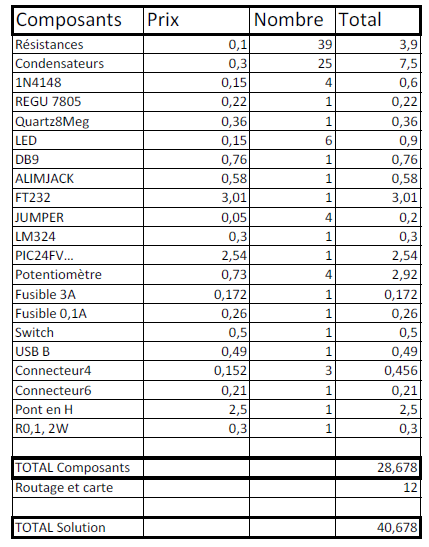
\includegraphics[width=15cm]{SolutionAnalogique/cout.png}
	\label{cout}
	\caption{Tableau répertoriant les composants utilisés et leurs coûts}
\end{figure}

\end{document}



